\documentclass{beamer}

\usefonttheme{structurebold}

\usepackage[utf8]{inputenc}
\usepackage[T1]{fontenc}
\usepackage[portuguese]{babel} 



\title{Kotlin: como começar}
\date{\today}
\author{Ricardo Peixoto Robaina \\ Tchelinux Bagé}
\institute{Universidade Federal do Pampa}

\usetheme{unipampa}




\begin{document}
	
	\begin{frame}[noframenumbering]
		\titlepage
		\thispagestyle{empty}
	\end{frame}
	
	\begin{frame}{Sumário}
		\setbeamertemplate{section in toc}[sections numbered]
		\tableofcontents[hideallsubsections]
	\end{frame}

\section{Introdução}
	\begin{frame}{Introdução}
		
		\begin{itemize}
			\item Linguagem de Programação
			\item JetBrains (2010)
			\item Open Source
			\item Estaticamente tipada
			\item Inspirada em linguagens como: Java, C#, JavaScript
			\item Paradigma:
				\begin{itemize}
					\item OO
					\item Funcional
				\end{itemize}
			
			\item \textbf{Multiplataforma}
		\end{itemize}
	
	\end{frame}

	\begin{frame}{Histórico}
		\begin{itemize}
			\item Java (90's)
			\item JetBrains
			\begin{figure}[!htb]
				\centering
				
\includegraphics[scale=.20]{jetBrains.png}
			\end{figure}
			\item Comunidade
			\item Google I/O 2017 - linguagem oficial de desenvolvimento Android
		\end{itemize}
	
	\end{frame}

\begin{frame}{Linhas de código Kotlin no Github}
	\begin{figure}[!htb]
		\centering
		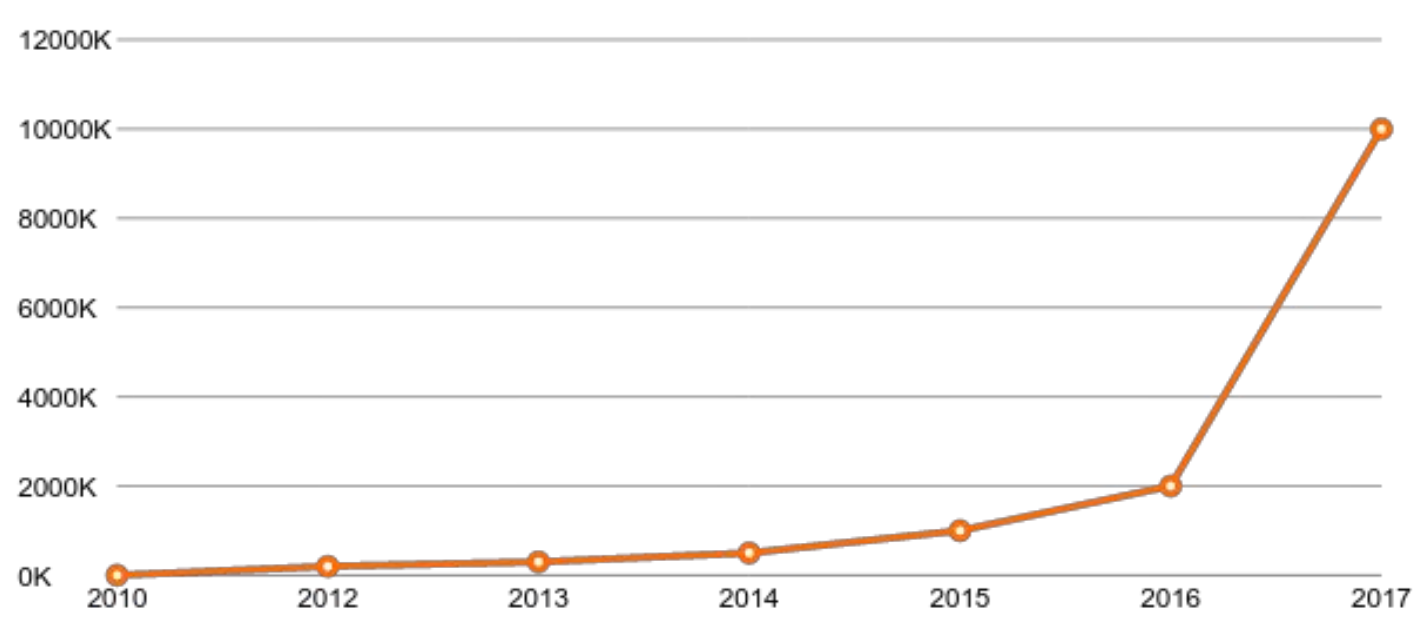
\includegraphics[scale=.2]{grafico.png}
	\end{figure}
\end{frame}

\section{Características}
\begin{frame}{Características}
	\begin{figure}[!htb]
		\centering
		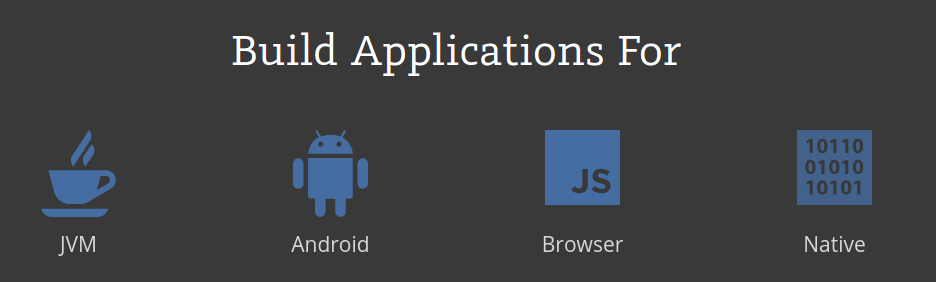
\includegraphics[scale=.25]{caracteristicas.png}
	\end{figure}
	
	\begin{figure}[!htb]
		\centering
		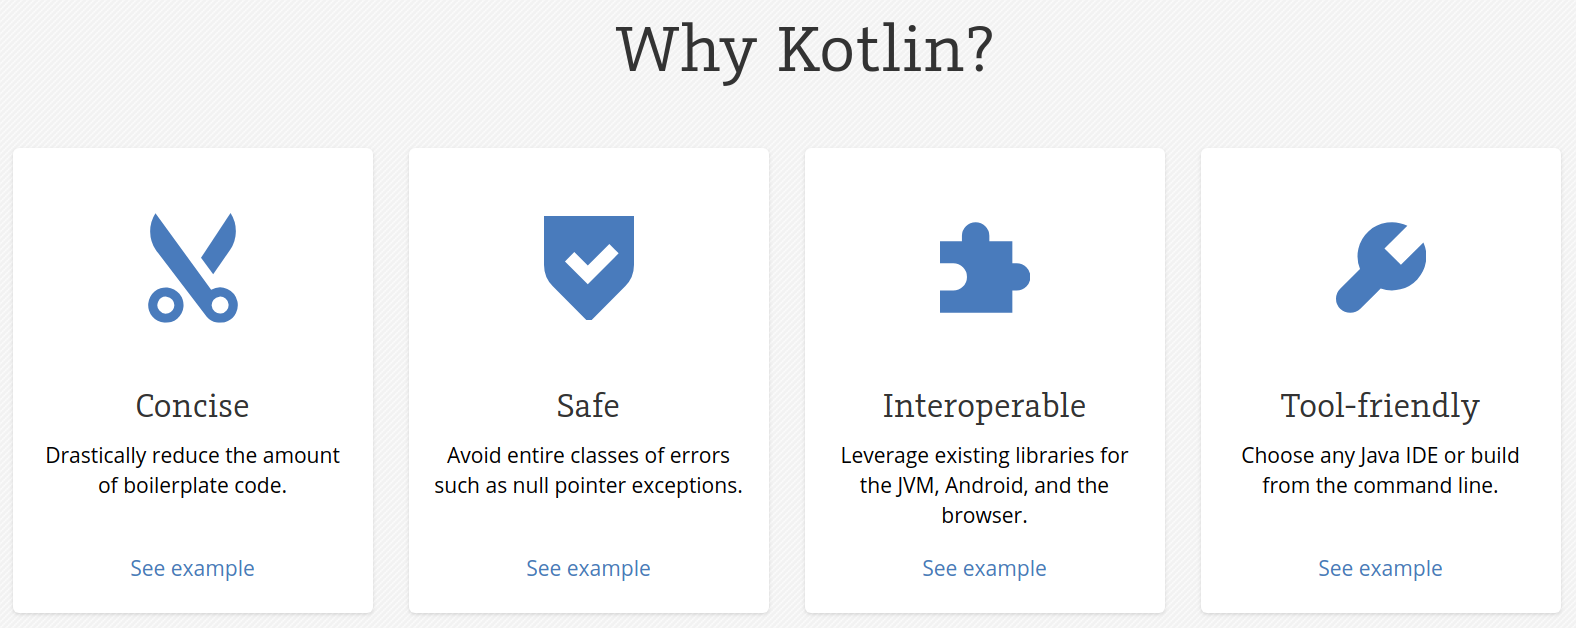
\includegraphics[scale=.20]{why.png}
	\end{figure}
	
\end{frame}



\section{Instalação}
\begin{frame}{Instalação}


	\begin{block}{SDKMAN!}
		\begin{itemize}
			\item \$ curl -s https://get.sdkman.io | bash
		\end{itemize}
	\end{block}

	\pause

	\begin{block}{Compilador (Kotlin)}
		\begin{itemize}
			 	\item \$ sdk install kotlin
		\end{itemize}
	\end{block}
	
	\pause
	
	\begin{block}{IntelliJ IDEA Community}
		\begin{figure}[!htb]
			\begin{itemize}
				\item https://www.jetbrains.com/idea/download/#section=linux5
			\end{itemize}
			
			\centering
			
\includegraphics[scale=.15]{intellij.png}
		\end{figure}
		
		
		
	\end{block}
	

\end{frame}

\begin{frame}{Try Kotlin}

	https://try.kotlinlang.org/
	
	\begin{figure}[!htb]
		\centering
		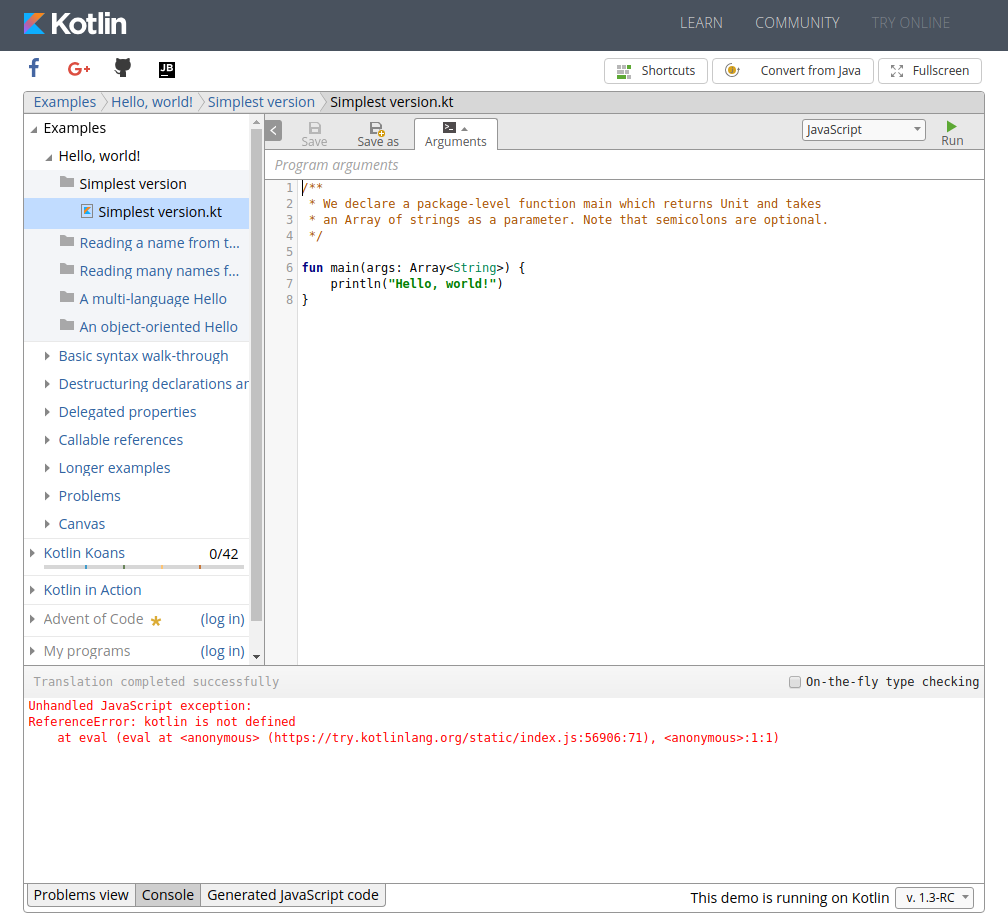
\includegraphics[scale=.20]{trykotlin.png}
	\end{figure}
	
	\begin{itemize}
		\item Koans
	\end{itemize}
	
\end{frame}





\section{Sintaxe básica}
	\begin{frame}{Sintaxe Básica}
		\begin{figure}[!htb]
			\centering
			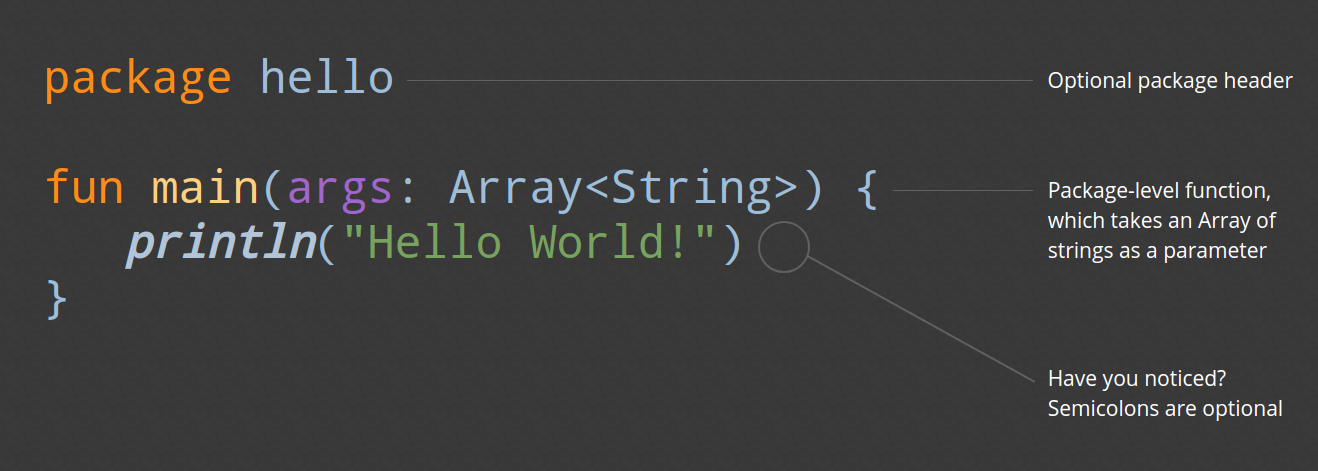
\includegraphics[scale=.23]{helloworld.png}
		\end{figure}
	\end{frame}

\begin{frame}{Compilação}
	\begin{itemize}
		\item hello.kt
		\item \$ kotlinc hello.kt -include-runtime -d hello.jar
		\item \$ java -jar hello.jar
	\end{itemize}
\end{frame}

\section{Interoperabilidade com Java}


\section{Desenvolvimento Android}
	\begin{frame}{Desenvolvimento Android}
		
		\begin{figure}[!htb]
			\centering
			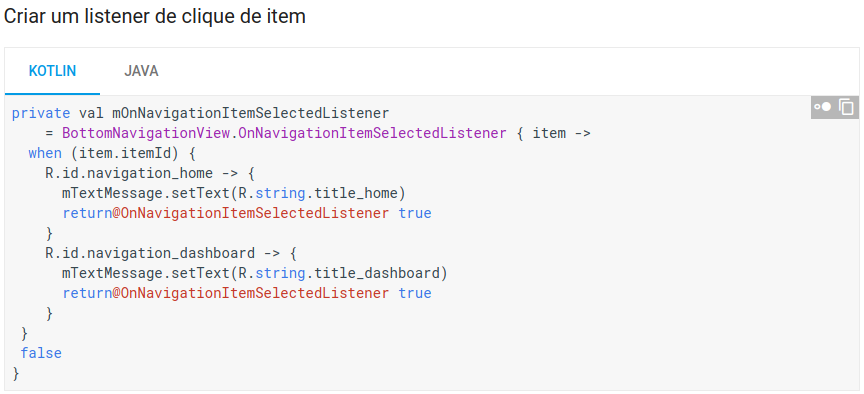
\includegraphics[scale=.3]{androidKotlin.png}
		\end{figure}
		
		
		\begin{figure}[!htb]
			\centering
			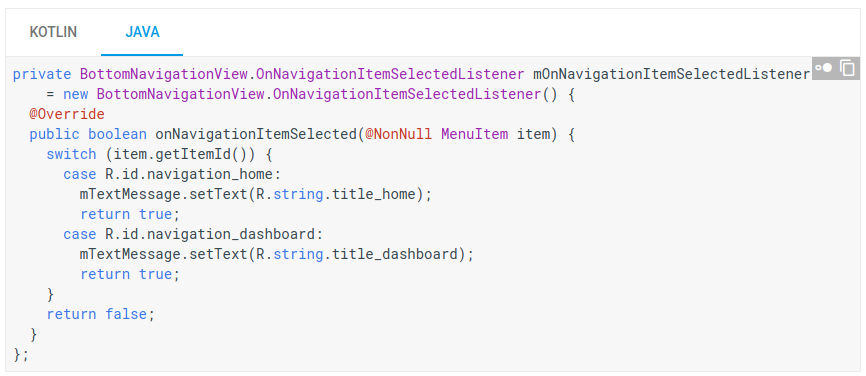
\includegraphics[scale=.3]{androidJava.png}
		\end{figure}
	
		
		
	\end{frame}



\section{Comunidade}

	\begin{frame}{Comunidade}
	
		\begin{figure}[!htb]
			\centering
			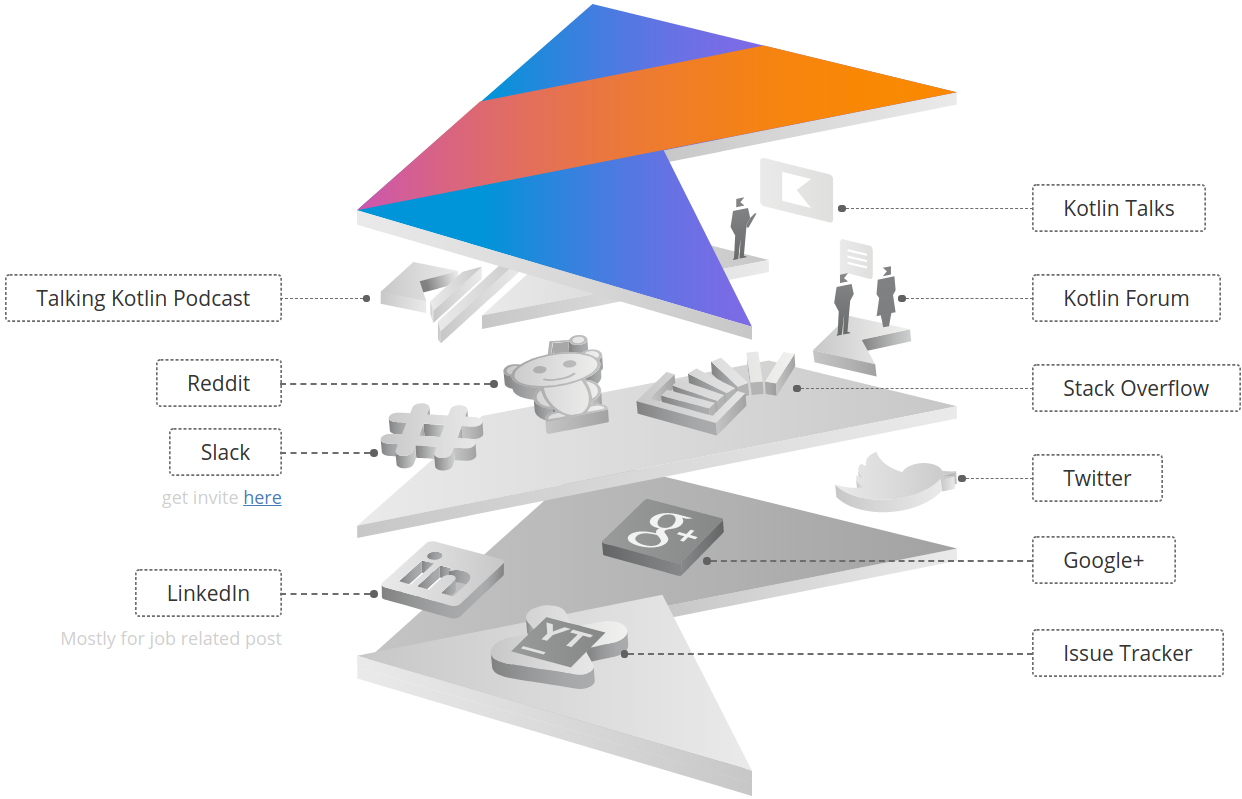
\includegraphics[scale=.23]{comunidade.png}
		\end{figure}
	
	https://kotlinlang.org/community/
	
	\end{frame}





\section{Referências}
	
\begin{frame}{Referências}
	
	
			\begin{itemize}
				\item https://kotlinlang.org/
				
				\item \textbf{Google I/O 2017} https://www.youtube.com/watch?v=X1RVYt2QKQE
				\\
				
\includegraphics[width=0.5\textwidth]{io17.png}
			
				\item \textbf{Google I/O 2018}  https://www.youtube.com/watch?v=6P20npkvcb8
				\\
				
\includegraphics[width=0.5\textwidth]{io18.png}
				
				
			\end{itemize}

	
	
\end{frame}

\begin{frame}{Kotlin: como começar}
	
		\newline
		\begin{center}
			{\Huge  \textbf{Obrigado!} \\}
		\end{center}
		
		{\normalsize 
			\begin{itemize}
				\item ricardorobaina11@gmail.com 
				\item https://github.com/robainaricardo/TchelinuxBage \\ \newline   
			\end{itemize}	
		}
		\maketitle
	
\end{frame}



\end{document}